\documentclass{jsarticle}
\usepackage{amsmath}
\usepackage[dvipdfmx]{graphicx}
\usepackage[dvipdfmx]{color}
\usepackage{mathtools}
\usepackage{physics}
\usepackage{siunitx}
\usepackage{wrapfig}
\usepackage{bm}
\mathtoolsset{showonlyrefs=true}

\begin{document}

\title{条件付き最適設計}
\author{前田陽祐(03-240236)}
\maketitle

\section{目的}
講義における例を参考に、ある体積をもつ円筒容器の設計を考える。
その際、円筒容器に使用する材料の体積を最小化することを目的とする。

\subsection{設計変数}
円筒容器の内側の半径${x_r}$と内側の高さ${x_h}$、容器の厚み$t$を設計変数とする。

\subsection{制約関数}
円筒容器の体積$V$が一定であるとする。
\begin{equation}
  h({x_r}, {x_h}) = \pi {x_r}^2 {x_h} - V = 0
\end{equation}

\subsection{目的関数}
円筒容器に使用する材料の体積$V_{\text{material}}$を最小化する。

材料力学より、円筒容器の内圧$p$に耐えられる容器の厚み$t$は内圧と外圧(大気圧)$p_0$の差$p-p_0$に比例する。
\begin{equation}
  t = \frac{(p-p_0) {x_r}}{\sigma}
\end{equation}
ここで、$\sigma$は材料の許容応力である。

また、内圧$p$の最大値は、容器の高さ${x_h}$と大気圧$p_0$によって決まる。
\begin{equation}
  p = p_0 + \rho g {x_h}
\end{equation}
ここで、$\rho$は液体の密度、$g$は重力加速度である。
したがって、内圧と外圧の差は次のように表される。
\begin{equation}
  p - p_0 = \rho g {x_h}
\end{equation}

円筒容器の面積は$2\pi {x_r}^2 + 2\pi {x_r} {x_h}$であるので、材料の体積は単純化して次のように表される。
\begin{align}
  V_{\text{material}} &= (2\pi {x_r}^2 + 2\pi {x_r} {x_h}) t \\
                      &=  2\pi {x_r} ({x_r}+{x_h}) \frac{(p-p_0) {x_r}}{\sigma} \\
                      &= \frac{2\pi\rho g }{\sigma} {x_r}^2 {x_h}({x_r}+{x_h})
\end{align}

目的関数は定数倍を無視することができるので、次のように表される。
\begin{equation}
  f({x_r}, {x_h}) = {x_r}^2 {x_h} ({x_r}+{x_h})
  = {x_r}^3h + {x_r}^2h^2
\end{equation}

\section{最適化}
\subsection{ラグランジュアン}
ラグランジュアン$L$は次のように表される。
\begin{align}
  L({x_r}, {x_h}, \lambda) &= f({x_r}, {x_h}) + \lambda h({x_r}, {x_h}) \\
                   &= {x_r}^3h + {x_r}^2h^2 + \lambda (\pi {x_r}^2 {x_h} - V)
\end{align}

\subsection{必要条件}
必要条件は${x_r}, {x_h}, \lambda$のそれぞれでのラグランジュアンの偏微分が$0$になることである。
すなわち、
\begin{align}
  \pdv{L}{{x_r}}&= 3r^2h + 2rh^2 + 2\pi\lambda rh
  =0 \label{eq:d-{x_r}} \\
  \pdv{L}{{x_h}}&= {x_r}^3 + 2r^2h + \pi\lambda {x_r}^2
  =0 \label{eq:d-h} \\ 
  \pdv{L}{\lambda}&= \pi {x_r}^2h-V
  =0.\label{eq:d-lambda}
\end{align}

\subsection{解}
式\eqref{eq:d-lambda}より、
\begin{equation}
  {x_h}=\frac{V}{\pi {x_r}^2}
  \label{eq:h-{x_r}}
\end{equation}
が得られる。
これを式\eqref{eq:d-h}に代入すると、
\begin{align}
  {x_r}^3 + 2r^2\frac{V}{\pi {x_r}^2} + \pi\lambda {x_r}^2 = 0 \\
  {x_r}^3 + \frac{2V}{\pi} + \pi\lambda {x_r}^2 = 0 \\
  \lambda = -\frac{{x_r}}{\pi} - \frac{2V}{\pi^2 {x_r}^2}
  \label{eq:lambda-{x_r}}
\end{align}
となる。これを式\eqref{eq:d-{x_r}}に代入して、
\begin{align}
  3r^2\cdot\frac{V}{\pi {x_r}^2} 
  + 2r\cdot\qty(\frac{V}{\pi {x_r}^2})^2 
  + 2\pi\qty(
    -\frac{{x_r}}{\pi} - \frac{2V}{\pi^2 {x_r}^2}
    )
    \cdot {x_r}\cdot
    \frac{V}{\pi {x_r}^2} = 0 \\
  3\frac{V}{\pi} 
  + 2\frac{V^2}{\pi^2 {x_r}^3} 
  - 2\frac{V}{\pi}
  - 4\frac{V^2}{\pi^2 {x_r}^3} = 0 \\
  \frac{V}{\pi} - 2\frac{V^2}{\pi^2 {x_r}^3} = 0 \\
  {x_r} = \sqrt[3]{\frac{2V}{\pi}}.
\end{align}
したがって、式\eqref{eq:h-{x_r}}より、
\begin{equation}
  {x_h} = \frac{V}{\pi {x_r}^2} 
  = \sqrt[3]{\frac{V}{4\pi}}.
\end{equation}
式\eqref{eq:lambda-{x_r}}より、
\begin{equation}
  \lambda = -\frac{{x_r}}{\pi} - \frac{2V}{\pi^2 {x_r}^2} 
  = -\sqrt[3]{\frac{2V}{\pi^4}} - \sqrt[3]{\frac{2V}{\pi^4}} 
  = -\sqrt[3]{\frac{16V}{\pi^4}}.
\end{equation}
これが最適解の候補である。

\subsection{十分条件}
ヘッシアン行列$H$は以下のように表される。
\begin{align}
  H &=
  \mqty[
  \pdv[2]{L}{{x_r}} & \pdv{L}{{x_r}}{{x_h}} \\
  \pdv{L}{{x_h}}{{x_r}} & \pdv[2]{L}{{x_h}} \\
  ]
  \\&=
  \mqty[
  6rh+2h^2+2\pi\lambda {x_h} & 3r^2+4rh+2\pi\lambda {x_r} \\
  3r^2+4rh+2\pi\lambda {x_r} & 2r^2 \\
  ]
\end{align}
これに最適解の候補
\begin{equation}
  \left\{ \,
  \begin{aligned}
     & {x_r} = \sqrt[3]{\frac{2V}{\pi}} \\
     & {x_h} = \sqrt[3]{\frac{V}{4\pi}} \\
     & \lambda = -\sqrt[3]{\frac{16V}{\pi^4}}
  \end{aligned}
  \right.
  \label{eq:canditate}
\end{equation}
を代入すると、
\begin{align}
  H&=
  \mqty[
  6\sqrt[3]{\frac{V^2}{2\pi^2}} + 2\sqrt[3]{\frac{V^2}{16\pi^2}} - 2\pi\sqrt[3]{\frac{4V^2}{\pi^5}} &
  3\sqrt[3]{\frac{4V^2}{\pi^2}} + 4\sqrt[3]{\frac{V^2}{2\pi^2}} - 2\pi\sqrt[3]{\frac{4V^2}{\pi^5}} \\
  3\sqrt[3]{\frac{4V^2}{\pi^2}} + 4\sqrt[3]{\frac{V^2}{2\pi^2}} - 2\pi\sqrt[3]{\frac{4V^2}{\pi^5}} &
  2\sqrt[3]{\frac{4V^2}{\pi^2}}
  ]\\
  &= \sqrt[3]{\frac{V^2}{\pi^2}}
  \mqty[
  \sqrt[3]{108} + \sqrt[3]{\frac{1}{2}} - \sqrt[3]{32} &
  \sqrt[3]{108} + \sqrt[3]{32} - \sqrt[3]{32} \\
  \sqrt[3]{108} + \sqrt[3]{32} - \sqrt[3]{32} &
  \sqrt[3]{108}
  ]\\
  &= \sqrt[3]{\frac{V^2}{\pi^2}}
  \mqty[
  \sqrt[3]{108} + \sqrt[3]{\frac{1}{2}} - \sqrt[3]{32} &
  \sqrt[3]{108} \\
  \sqrt[3]{108} &
  \sqrt[3]{108}
  ]
  \label{eq:H-val}
\end{align}
これを用いて、最適解の十分条件
$\partial{x}^*H\partial{x}>0 \text{ for }\forall\partial x\neq 0$
について考える。
\begin{align}
  \partial{x}^*H\partial{x}
  / \sqrt[3]{\frac{V^2}{\pi^2}}
  &= 
  \mqty[\partial{{x_r}} & \partial{{x_h}}]
  \mqty[
  \sqrt[3]{108} + \sqrt[3]{\frac{1}{2}} - \sqrt[3]{32} &
  \sqrt[3]{108} \\
  \sqrt[3]{108} &
  \sqrt[3]{108}
  ]
  \mqty[\partial{{x_r}} \\ \partial{{x_h}}] \\
  &=
  \qty(\sqrt[3]{108} + \sqrt[3]{\frac{1}{2}} - \sqrt[3]{32}) \cdot (\partial{{x_r}})^2
  + 2\qty(\sqrt[3]{108}) \cdot \partial{{x_r}}\partial{{x_h}}
  + \qty(\sqrt[3]{108}) \cdot (\partial{{x_h}})^2
\end{align}
ここで、$h=0$の条件より、以下の式を用いることができる。
\begin{equation}
  \nabla h \cdot \partial x = \mqty[\pdv{h}{{x_r}} & \pdv{h}{{x_h}}] \mqty[\partial{{x_r}} \\ \partial{{x_h}}] = 
  2\pi {x_r} {x_h} \partial{{x_r}} + \pi {x_r}^2 \partial{{x_h}} = 0
\end{equation}
これに最適解の候補\eqref{eq:canditate}を代入すると、
\begin{equation}
  2\pi {x_r} {x_h} \partial{{x_r}} + \pi {x_r}^2 \partial{{x_h}} 
  = 2\pi \sqrt[3]{\frac{V^2}{2\pi^2}} \partial{{x_r}} + \pi \sqrt[3]{\frac{4V^2}{\pi^2}} \partial{{x_h}}
  = 0
\end{equation}
したがって、
\begin{equation}
  \partial{{x_h}} = -\partial{{x_r}}
\end{equation}
を得る。これを用いて、
\begin{align}
  \partial{x}^*H\partial{x}
  / \sqrt[3]{\frac{V^2}{\pi^2}}
  &=
  \qty(\sqrt[3]{108} + \sqrt[3]{\frac{1}{2}} - \sqrt[3]{32}) \cdot (\partial{{x_r}})^2
  + 2\qty(\sqrt[3]{108}) \cdot \partial{{x_r}}(-\partial{{x_r}})
  + \qty(\sqrt[3]{108}) \cdot (-\partial{{x_r}})^2 \\
  &=\qty(\sqrt[3]{\frac{1}{2}} - \sqrt[3]{32}) \cdot (\partial{{x_r}})^2 
  < 0
\end{align}
という結果になる。
したがって、最適解の候補\eqref{eq:canditate}は最適解ではないことがわかる。

\section{考察}
最適解の候補\eqref{eq:canditate}は最適解ではないことがわかった。
この結果を簡単なグラフと比較して考察する。
$V=\pi$としたときの$f({x_r}, {x_h})$のグラフを図\ref{fig:f}に示す。
このグラフを見ると、最適解の候補\eqref{eq:canditate}の値($x_r\approx 1.3$)に極小値が存在することがわかる。
したがって、上記の十分条件に関する議論には誤りがあり、最適解の候補\eqref{eq:canditate}は最適解であると考えられる。
\begin{figure}[b]
  \centering
  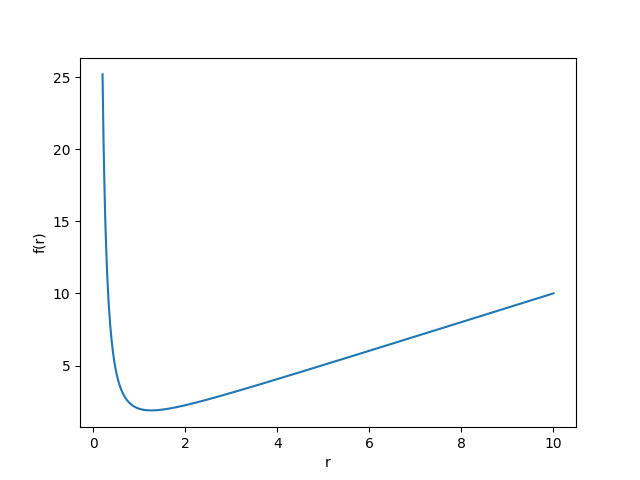
\includegraphics[width=\textwidth]{./graph/graph.png}
  \caption{$f({x_r}, {x_h})$のグラフ}
  \label{fig:f}
\end{figure}
\end{document}
